To be able to identify the balls, the location of each ball is needed. By knowing where the balls are placed, features from each ball can be extracted and compared for identification.

The location of a ball is defined by the position of the bounding circle of the ball. The radius of a ball is equal  and known for all balls\fxnote{Maybe we should define that it is found by some kind of calibration.}, and the balls can then be represented by the center point alone.

The located positions must be precise to gain the optimal working conditions for the identifier. A ball location that is slightly shifted will result in a ball region that contains pixels which does not come from the ball. This will make it harder for the identifier to identify the ball, and it will become even harder if the region intersects another ball because the region will then become a mix of two different balls. This can cause that the two balls are classified as the other and thereby 2 identification errors.

\subsubsection{Preliminary segmentation}
To decrease the ROI from the cloth area down to areas of the table that contains balls, a preliminary segmentation is performed. A color threshold removes all pixels that belong to the background leaving behind a mask that represents the balls.
\begin{figure}[h]
  \centering
  \subfloat[Before]{\label{fig:gull}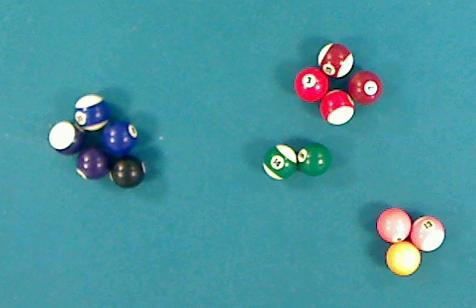
\includegraphics[width=0.48\textwidth]{images/thres1before.jpg}}
  \quad           
  \subfloat[After]{\label{fig:tiger}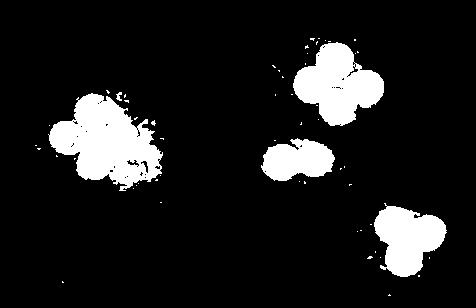
\includegraphics[width=0.48\textwidth]{images/thres1after.jpg}}
   \caption{Color threshold to remove background}
  \label{fig:thres1}
\end{figure}
Figure \ref{fig:thres1} shows the result of the color threshold. In a situation like this where the balls are laying close to each other, the preliminary segmentation is not enough to successfully separate the balls. Balls in close proximity results in connected BLOBs after the threshold. These BLOBs could be separated using morphology operations but most of the information would be lost, causing the locations to lack precision. Instead of using the BLOBS directly, they are used as search regions for the balls.

\subsubsection{Background cross-correlation}
To get a precise ball position, the cross-correlation between the table image and a ball shaped patch of the background is computed. The idea is that the positions that has the lowest correlation will be ball positions. The background patch is constructed by drawing a filled circle which has the same radius as a ball. The circle is placed in a transparent image to prevent computation of cross-correlation outside of the circle. By using a circular patch, the system is able to get a better match against circular regions like the balls.

FIGURE SHOWING CORRELATION

The correlation will have several points with low value in the area around a ball center. To prevent the same ball from being matched more than once, we utilize the knowledge that balls can not intersect with one another. The first ball is found at the position of the minimum in the correlation image. The position and the area around it corresponding to the radius is then marked as matched. The next ball can then not be found any closer than one radius from the previous matches. A problem arises if a wrong match is found which intersects a not matched ball. It will then be impossible to find a new match in the region of the earlier wrong match.
Figure \ref{fig:wronglocate} shows the problem of a wrong match. The wrong match prevents several balls from being matched, and other balls from matching precisely.
\begin{figure}[h]
\begin{center}
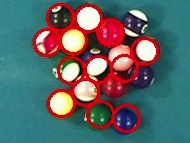
\includegraphics{images/wronglocate.jpg}
\caption{Consequence of wrong location match. Red circles are ball matches}
\label{fig:wronglocate}
\end{center}
\end{figure}